\documentclass[letterpaper,11pt]{article}

\usepackage{geometry}
\usepackage{pslatex}
\usepackage{fancyhdr}
\usepackage{graphicx}
\usepackage{color}
\usepackage{tikz}
\usepackage{setspace}
\usepackage{amssymb}

\geometry{ margin = 1.0in }

\pagestyle{fancy}
\lhead{{\bf Lecture 36}}
\chead{{\bf CMPSC 465 Fall 2020}}
\rhead{{\bf Mingfu Shao}}

\setlength\parindent{0em}
\setlength\parskip{8pt}
%\setlength{\fboxsep}{6pt}

\usepackage{amsthm}
\newtheoremstyle{mytheorem}
  {\parskip} % Space above
  {0em} % Space below
  {} % Body font
  {} % Indent amount
  {\bfseries} % Theorem head font
  {.} % Punctuation after theorem head
  {.5em} % Space after theorem head
  {} % Theorem head spec (can be left empty, meaning `normal')

\theoremstyle{mytheorem}
\newtheorem{definition}{Definition}
\newtheorem{property}{Property}
\newtheorem{claim}{Claim}
\newtheorem{fact}{Fact}
\newtheorem{corollary}{Corollary}

% for algorithms
\newcommand{\aaa}[1]{\hspace{0.65cm}\parbox[t]{15.3cm}{#1}}
\newcommand{\aab}[1]{\hspace{1.15cm}\parbox[t]{15.0cm}{#1}}
\newcommand{\aac}[1]{\hspace{1.65cm}\parbox[t]{15.0cm}{#1}}
\newcommand{\aad}[1]{\hspace{2.15cm}\parbox[t]{15.0cm}{#1}}
\newcommand{\aae}[1]{\hspace{2.65cm}\parbox[t]{15.0cm}{#1}}
\newcommand{\aaf}[1]{\hspace{3.15cm}\parbox[t]{15.0cm}{#1}}
\newcommand{\aaA}[2]{\hspace{0.5cm} {\tikz[overlay] \draw (0.1, -0.1) -- (0.1, #1 * -1.5em + 0.6em);} \parbox[t]{15.0cm}{#2}}
\newcommand{\aaB}[2]{\hspace{1.0cm} {\tikz[overlay] \draw (0.1, -0.1) -- (0.1, #1 * -1.5em + 0.6em);} \parbox[t]{15.0cm}{#2}}
\newcommand{\aaC}[2]{\hspace{1.5cm} {\tikz[overlay] \draw (0.1, -0.1) -- (0.1, #1 * -1.5em + 0.6em);} \parbox[t]{15.0cm}{#2}}
\newcommand{\aaD}[2]{\hspace{2.0cm} {\tikz[overlay] \draw (0.1, -0.1) -- (0.1, #1 * -1.5em + 0.6em);} \parbox[t]{15.0cm}{#2}}
\newcommand{\aaE}[2]{\hspace{2.5cm} {\tikz[overlay] \draw (0.1, -0.1) -- (0.1, #1 * -1.5em + 0.6em);} \parbox[t]{15.0cm}{#2}}
\newcommand{\xxx}{\par\vspace{0.1cm}}

\begin{document}

\section*{Network Flow}

A \emph{network}~(also called \emph{flow network}) models 
an abstracted flow~(traffic, data, etc) transmits from an origin to a destination
via a graphical structure. Formally, a (flow) network is a tuple $(G = (V, E), s, t, c(\cdot))$, where
%$G = (V, E)$ is a directed graph, $s\in V$ represents the source vertex~(i.e., the in-degree of $s$ is 0),
%$t\in V$ represents the sink vertex~(i.e., the out-degree of $t$ is 0),
%and $c(e) \ge 0$ represents the \emph{capacity} of edge $e\in E$.

\vspace*{-\topsep}
\begin{enumerate}
\item $G = (V, E)$ is a directed graph;
\item $s\in V$ is a source vertex of $G$~(i.e., the in-degree of $s$ is 0), from which the flow is generated;
\item $t\in V$ is a sink vertex of $G$~(i.e., the out-degree of $t$ is 0), at which the flow is absorbed;
\item $c: E\to \mathbb{R}^+$, in which $c(e)$ represents the \emph{capacity} of edge $e\in E$, which models the limit of the flow that edge $e$ can carry.
\end{enumerate}

An \emph{$s$-$t$ flow} of network $(G = (V, E), s, t, c(\cdot))$
describes {how} the flow is transmitted from $s$ to $t$
via the graph $G$ under the capacity constraints. Formally,
an $s$-$t$ flow $f$ is a function $f: E\to \mathbb{R}^+$
that satisfies the following two conditions:
\vspace*{-\topsep}
\begin{enumerate}
\item For every $e\in E$, $0\le f(e) \le c(e)$; this is called the \emph{capacity condition};
\item For every vertex $v\in V\setminus\{s,t\}$, $\sum_{e\in I(v)} f(e) = \sum_{e\in O(v)} f(e)$, where $I(v) := \{(u,v)\in E\mid u\in V\}$ represents
the set of in-edges of $v$, and $O(v) := \{(v,w)\in E\mid w\in V\}$ represents
the set of out-edges of $v$. This is called the \emph{conservation condition}.
\end{enumerate}

Intuitively, an $s$-$t$ flow assigns an non-negative value $f(e)$ to edge $e$, representing the
amount of flow that is carried by edge $e$; such amount must not exceed the capacity of $e$, i.e., $f(e) \le c(e)$, for every $e\in E$.
All vertices, except the source $s$ that generates the flow and the sink that absorbs the flow,
redistribute the flow~(instead of repositing any flow); therefore, for each vertex $v\in V\setminus\{s,t\}$,
the total amount of flow that enters $v$ equals to the total amount of flow that leaves $v$.
See Figure~\ref{fig:flow}.

\begin{figure}[h]
\centering{

\tikzset{every picture/.style={line width=0.75pt}} %set default line width to 0.75pt        

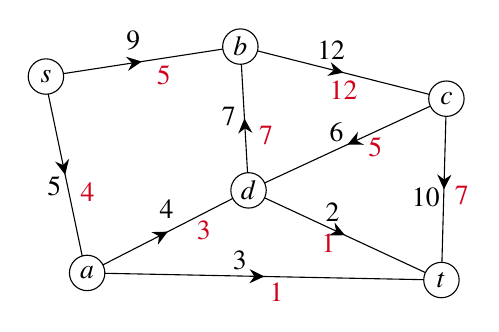
\begin{tikzpicture}[x=0.5pt,y=0.5pt,yscale=-1,xscale=1]
%uncomment if require: \path (0,222); %set diagram left start at 0, and has height of 222

%Straight Lines [id:da3853598268579197] 
\draw    (24.79,46.83) -- (165.31,25.18) ;
\draw [shift={(95.05,36)}, rotate = 531.24] [fill={rgb, 255:red, 0; green, 0; blue, 0 }  ][line width=0.08]  [draw opacity=0] (10.72,-5.15) -- (0,0) -- (10.72,5.15) -- (7.12,0) -- cycle    ;
%Straight Lines [id:da6958538828947681] 
\draw    (24.79,46.83) -- (54.58,188.77) ;
\draw [shift={(39.69,117.8)}, rotate = 258.15] [fill={rgb, 255:red, 0; green, 0; blue, 0 }  ][line width=0.08]  [draw opacity=0] (10.72,-5.15) -- (0,0) -- (10.72,5.15) -- (7.12,0) -- cycle    ;
%Straight Lines [id:da2980592918523626] 
\draw    (55.58,188.77) -- (311.62,193.9) ;
\draw [shift={(183.6,191.34)}, rotate = 181.15] [fill={rgb, 255:red, 0; green, 0; blue, 0 }  ][line width=0.08]  [draw opacity=0] (10.72,-5.15) -- (0,0) -- (10.72,5.15) -- (7.12,0) -- cycle    ;
%Straight Lines [id:da14604600957867897] 
\draw    (172.22,129.11) -- (311.62,193.9) ;
\draw [shift={(241.92,161.5)}, rotate = 204.92000000000002] [fill={rgb, 255:red, 0; green, 0; blue, 0 }  ][line width=0.08]  [draw opacity=0] (10.72,-5.15) -- (0,0) -- (10.72,5.15) -- (7.12,0) -- cycle    ;
%Straight Lines [id:da8640956582518242] 
\draw    (166.31,25.18) -- (172.22,129.11) ;
\draw [shift={(169.27,77.14)}, rotate = 86.75] [fill={rgb, 255:red, 0; green, 0; blue, 0 }  ][line width=0.08]  [draw opacity=0] (10.72,-5.15) -- (0,0) -- (10.72,5.15) -- (7.12,0) -- cycle    ;
%Straight Lines [id:da285469110869773] 
\draw    (166.31,25.18) -- (315.22,62.84) ;
\draw [shift={(240.76,44.01)}, rotate = 194.2] [fill={rgb, 255:red, 0; green, 0; blue, 0 }  ][line width=0.08]  [draw opacity=0] (10.72,-5.15) -- (0,0) -- (10.72,5.15) -- (7.12,0) -- cycle    ;
%Straight Lines [id:da8162300663234149] 
\draw    (315.22,62.84) -- (311.62,193.9) ;
\draw [shift={(313.42,128.37)}, rotate = 271.57] [fill={rgb, 255:red, 0; green, 0; blue, 0 }  ][line width=0.08]  [draw opacity=0] (10.72,-5.15) -- (0,0) -- (10.72,5.15) -- (7.12,0) -- cycle    ;
%Straight Lines [id:da5085854502811855] 
\draw    (315.22,62.84) -- (172.22,129.11) ;
\draw [shift={(243.72,95.98)}, rotate = 335.13] [fill={rgb, 255:red, 0; green, 0; blue, 0 }  ][line width=0.08]  [draw opacity=0] (10.72,-5.15) -- (0,0) -- (10.72,5.15) -- (7.12,0) -- cycle    ;
%Straight Lines [id:da4064365628912957] 
\draw    (172.22,129.11) -- (55.58,188.77) ;
\draw [shift={(113.9,158.94)}, rotate = 152.91] [fill={rgb, 255:red, 0; green, 0; blue, 0 }  ][line width=0.08]  [draw opacity=0] (10.72,-5.15) -- (0,0) -- (10.72,5.15) -- (7.12,0) -- cycle    ;
%Shape: Ellipse [id:dp651117123053256] 
\draw  [fill={rgb, 255:red, 255; green, 255; blue, 255 }  ,fill opacity=1 ] (13,46.83) .. controls (13,39.77) and (18.73,34.04) .. (25.79,34.04) .. controls (32.86,34.04) and (38.58,39.77) .. (38.58,46.83) .. controls (38.58,53.9) and (32.86,59.62) .. (25.79,59.62) .. controls (18.73,59.62) and (13,53.9) .. (13,46.83) -- cycle ;
%Shape: Ellipse [id:dp7399561756845123] 
\draw  [fill={rgb, 255:red, 255; green, 255; blue, 255 }  ,fill opacity=1 ] (153.52,25.18) .. controls (153.52,18.11) and (159.25,12.39) .. (166.31,12.39) .. controls (173.38,12.39) and (179.1,18.11) .. (179.1,25.18) .. controls (179.1,32.24) and (173.38,37.97) .. (166.31,37.97) .. controls (159.25,37.97) and (153.52,32.24) .. (153.52,25.18) -- cycle ;
%Shape: Ellipse [id:dp8268258265249401] 
\draw  [fill={rgb, 255:red, 255; green, 255; blue, 255 }  ,fill opacity=1 ] (302.43,62.84) .. controls (302.43,55.78) and (308.15,50.05) .. (315.22,50.05) .. controls (322.28,50.05) and (328.01,55.78) .. (328.01,62.84) .. controls (328.01,69.9) and (322.28,75.63) .. (315.22,75.63) .. controls (308.15,75.63) and (302.43,69.9) .. (302.43,62.84) -- cycle ;
%Shape: Ellipse [id:dp5421818862330341] 
\draw  [fill={rgb, 255:red, 255; green, 255; blue, 255 }  ,fill opacity=1 ] (159.43,129.11) .. controls (159.43,122.05) and (165.15,116.32) .. (172.22,116.32) .. controls (179.28,116.32) and (185.01,122.05) .. (185.01,129.11) .. controls (185.01,136.18) and (179.28,141.9) .. (172.22,141.9) .. controls (165.15,141.9) and (159.43,136.18) .. (159.43,129.11) -- cycle ;
%Shape: Ellipse [id:dp45600813719389455] 
\draw  [fill={rgb, 255:red, 255; green, 255; blue, 255 }  ,fill opacity=1 ] (42.79,188.77) .. controls (42.79,181.71) and (48.52,175.98) .. (55.58,175.98) .. controls (62.64,175.98) and (68.37,181.71) .. (68.37,188.77) .. controls (68.37,195.84) and (62.64,201.56) .. (55.58,201.56) .. controls (48.52,201.56) and (42.79,195.84) .. (42.79,188.77) -- cycle ;
%Shape: Ellipse [id:dp031187496945339066] 
\draw  [fill={rgb, 255:red, 255; green, 255; blue, 255 }  ,fill opacity=1 ] (298.83,193.9) .. controls (298.83,186.83) and (304.56,181.11) .. (311.62,181.11) .. controls (318.69,181.11) and (324.41,186.83) .. (324.41,193.9) .. controls (324.41,200.96) and (318.69,206.69) .. (311.62,206.69) .. controls (304.56,206.69) and (298.83,200.96) .. (298.83,193.9) -- cycle ;

% Text Node
\draw (25.79,46.83) node   [align=left] {$\displaystyle s$};
% Text Node
\draw (166.31,25.18) node   [align=left] {$\displaystyle b$};
% Text Node
\draw (315.22,62.84) node   [align=left] {$\displaystyle c$};
% Text Node
\draw (172.22,129.11) node   [align=left] {$\displaystyle d$};
% Text Node
\draw (55.58,188.77) node   [align=left] {$\displaystyle a$};
% Text Node
\draw (311.62,193.9) node   [align=left] {$\displaystyle t$};
% Text Node
\draw (229,48) node [anchor=north west][inner sep=0.75pt]   [align=left] {$\displaystyle \textcolor[rgb]{0.82,0.01,0.11}{12}$};
% Text Node
\draw (25,117) node [anchor=north west][inner sep=0.75pt]   [align=left] {$\displaystyle 5$};
% Text Node
\draw (106,134) node [anchor=north west][inner sep=0.75pt]   [align=left] {$\displaystyle 4$};
% Text Node
\draw (185.6,194.34) node [anchor=north west][inner sep=0.75pt]   [align=left] {$\displaystyle \textcolor[rgb]{0.82,0.01,0.11}{1}$};
% Text Node
\draw (82,12) node [anchor=north west][inner sep=0.75pt]   [align=left] {$\displaystyle 9$};
% Text Node
\draw (229,78) node [anchor=north west][inner sep=0.75pt]   [align=left] {$\displaystyle 6$};
% Text Node
\draw (151,67) node [anchor=north west][inner sep=0.75pt]   [align=left] {$\displaystyle 7$};
% Text Node
\draw (226,136) node [anchor=north west][inner sep=0.75pt]   [align=left] {$\displaystyle 2$};
% Text Node
\draw (319.42,124.37) node [anchor=north west][inner sep=0.75pt]   [align=left] {$\displaystyle \textcolor[rgb]{0.82,0.01,0.11}{7}$};
% Text Node
\draw (133,149) node [anchor=north west][inner sep=0.75pt]   [align=left] {$\displaystyle \textcolor[rgb]{0.82,0.01,0.11}{3}$};
% Text Node
\draw (223,159) node [anchor=north west][inner sep=0.75pt]   [align=left] {$\displaystyle \textcolor[rgb]{0.82,0.01,0.11}{1}$};
% Text Node
\draw (257,89) node [anchor=north west][inner sep=0.75pt]   [align=left] {$\displaystyle \textcolor[rgb]{0.82,0.01,0.11}{5}$};
% Text Node
\draw (178,81) node [anchor=north west][inner sep=0.75pt]   [align=left] {$\displaystyle \textcolor[rgb]{0.82,0.01,0.11}{7}$};
% Text Node
\draw (288.42,125.37) node [anchor=north west][inner sep=0.75pt]   [align=left] {$\displaystyle 10$};
% Text Node
\draw (220,19) node [anchor=north west][inner sep=0.75pt]   [align=left] {$\displaystyle 12$};
% Text Node
\draw (49,122) node [anchor=north west][inner sep=0.75pt]   [align=left] {$\displaystyle \textcolor[rgb]{0.82,0.01,0.11}{4}$};
% Text Node
\draw (104,37) node [anchor=north west][inner sep=0.75pt]   [align=left] {$\displaystyle \textcolor[rgb]{0.82,0.01,0.11}{5}$};
% Text Node
\draw (159,171) node [anchor=north west][inner sep=0.75pt]   [align=left] {$\displaystyle 3$};


\end{tikzpicture}

}
\caption{An example of a network and an $s$-$t$ flow.
The capacities are marked as black numbers next to edges;
the flow values are marked as red numbers next to edges.}
\label{fig:flow}
\end{figure}

The \emph{value} of an $s$-$t$ flow $f$, denoted as $|f|$,
is defined as the total amount of flow that is generated from source vertex $s$:
$|f| := \sum_{e\in O(s)} f(e)$. Intuitively, the total amount of flow that is generated
from $s$ eventually must be fully absorbed by sink $t$, as all internal vertex~(i.e., $V\setminus\{s,t\}$)
don't keep any flow. Therefore, we must have that 
$|f| = \sum_{e\in I(t)} f(e)$.  
This property is also a direct consequence of the conservation property.
Below we formally state and prove it.

\begin{fact}
We have $\sum_{e\in O(s)} f(e) = \sum_{e\in I(t)} f(e)$. 
\end{fact}

\emph{Proof.} According to the conservation condition:
$\sum_{e\in I(v)} f(e) = \sum_{e\in O(v)} f(e)$, 
for every vertex $v\in V\setminus\{s,t\}$. 
We sum up both sides over all $v\in V\setminus\{s,t\}$: 
we have $\sum_{v\in V\setminus\{s,t\}} \sum_{e\in I(v)} f(e) = \sum_{v\in V\setminus\{s,t\}} \sum_{e\in O(v)} f(e)$. 

We now break down the left side 
$L := \sum_{v\in V\setminus\{s,t\}} \sum_{e\in I(v)} f(e) 
= \sum_{v\in V} \sum_{e\in I(v)} f(e) -  \sum_{e\in I(s)} f(e) - \sum_{e\in I(t)} f(e)$.
Notice also that $\sum_{v\in V} \sum_{e\in I(v)} f(e) = \sum_{e\in E} f(e)$.
Since $s$ is a source vertex, we have $I(s) = \emptyset$, and therefore $\sum_{e\in I(s)} f(e)  = 0$.
Hence, $L = \sum_{e\in E} f(e) - \sum_{e\in I(t)} f(e)$.

Similarly, the right side 
$R := \sum_{v\in V\setminus\{s,t\}} \sum_{e\in O(v)} f(e) 
= \sum_{v\in V} \sum_{e\in O(v)} f(e) -  \sum_{e\in O(s)} f(e) - \sum_{e\in O(t)} f(e)$.
Again we have $\sum_{v\in V} \sum_{e\in O(v)} f(e) = \sum_{e\in E} f(e)$.
Since $t$ is a sink, we have $O(t) = \emptyset$, and therefore $\sum_{e\in O(t)} f(e)  = 0$.
Hence, $R = \sum_{e\in E} f(e) - \sum_{e\in O(s)} f(e)$.

Combining $L = R$ and noticing that $\sum_{e\in E} f(e)$ is shared, we have $\sum_{e\in O(s)} f(e) = \sum_{e\in I(t)} f(e)$, as desired.  \qed

We now define the \emph{maximum-flow problem}: given network $(G= (V, E), s, t, c(\cdot))$,
to find an $s$-$t$ flow $f$ such that $|f|$ is maximized.

See Figure~\ref{fig:maxflow} for an example. Playing with the instance you may find
a flow $f$ with $|f| = 9$, shown with red numbers in the figure.
It seems that this flow $f$ is a maximum flow.
Here is an argument that this flow $f$ is indeed a maximum flow.
Consider the \emph{cut} shown with blue curve. Notice that
$s$ and $t$ are on different sides of this cut. Therefore, all flow
from $s$ to $t$ must cross this cut. Notice also that there are three
cut-edges~(i.e., edges cross the border from $s$-side to $t$-side)
and the \emph{total capacities} of these 3 edges is $3 + 2 + 4 = 9$.
This gives an \emph{upper bound} of the maximum flow, which is 9.
And, we have found a flow $f$ with $|f| = 9$. Therefore, $f$
is a maximum flow.

\begin{figure}[h]
\centering{

\tikzset{every picture/.style={line width=0.75pt}} %set default line width to 0.75pt        

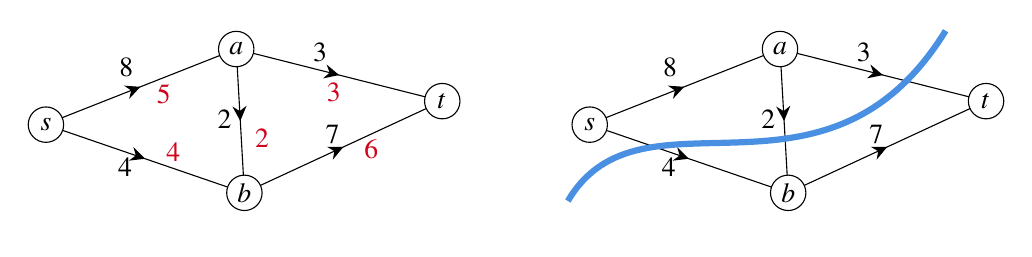
\begin{tikzpicture}[x=0.5pt,y=0.5pt,yscale=-1,xscale=1]
%uncomment if require: \path (0,166); %set diagram left start at 0, and has height of 166

%Straight Lines [id:da3853598268579197] 
\draw    (26.79,81.83) -- (165.31,27.18) ;
\draw [shift={(96.05,54.5)}, rotate = 518.47] [fill={rgb, 255:red, 0; green, 0; blue, 0 }  ][line width=0.08]  [draw opacity=0] (10.72,-5.15) -- (0,0) -- (10.72,5.15) -- (7.12,0) -- cycle    ;
%Straight Lines [id:da14604600957867897] 
\draw    (27.79,81.83) -- (171.22,131.11) ;
\draw [shift={(99.51,106.47)}, rotate = 198.96] [fill={rgb, 255:red, 0; green, 0; blue, 0 }  ][line width=0.08]  [draw opacity=0] (10.72,-5.15) -- (0,0) -- (10.72,5.15) -- (7.12,0) -- cycle    ;
%Straight Lines [id:da8640956582518242] 
\draw    (165.31,27.18) -- (171.22,131.11) ;
\draw [shift={(168.27,79.14)}, rotate = 266.75] [fill={rgb, 255:red, 0; green, 0; blue, 0 }  ][line width=0.08]  [draw opacity=0] (10.72,-5.15) -- (0,0) -- (10.72,5.15) -- (7.12,0) -- cycle    ;
%Straight Lines [id:da285469110869773] 
\draw    (165.31,27.18) -- (314.22,64.84) ;
\draw [shift={(239.76,46.01)}, rotate = 194.2] [fill={rgb, 255:red, 0; green, 0; blue, 0 }  ][line width=0.08]  [draw opacity=0] (10.72,-5.15) -- (0,0) -- (10.72,5.15) -- (7.12,0) -- cycle    ;
%Straight Lines [id:da5085854502811855] 
\draw    (314.22,64.84) -- (171.22,131.11) ;
\draw [shift={(242.72,97.98)}, rotate = 155.13] [fill={rgb, 255:red, 0; green, 0; blue, 0 }  ][line width=0.08]  [draw opacity=0] (10.72,-5.15) -- (0,0) -- (10.72,5.15) -- (7.12,0) -- cycle    ;
%Shape: Ellipse [id:dp651117123053256] 
\draw  [fill={rgb, 255:red, 255; green, 255; blue, 255 }  ,fill opacity=1 ] (15,81.83) .. controls (15,74.77) and (20.73,69.04) .. (27.79,69.04) .. controls (34.86,69.04) and (40.58,74.77) .. (40.58,81.83) .. controls (40.58,88.9) and (34.86,94.62) .. (27.79,94.62) .. controls (20.73,94.62) and (15,88.9) .. (15,81.83) -- cycle ;
%Shape: Ellipse [id:dp7399561756845123] 
\draw  [fill={rgb, 255:red, 255; green, 255; blue, 255 }  ,fill opacity=1 ] (152.52,27.18) .. controls (152.52,20.11) and (158.25,14.39) .. (165.31,14.39) .. controls (172.38,14.39) and (178.1,20.11) .. (178.1,27.18) .. controls (178.1,34.24) and (172.38,39.97) .. (165.31,39.97) .. controls (158.25,39.97) and (152.52,34.24) .. (152.52,27.18) -- cycle ;
%Shape: Ellipse [id:dp8268258265249401] 
\draw  [fill={rgb, 255:red, 255; green, 255; blue, 255 }  ,fill opacity=1 ] (301.43,64.84) .. controls (301.43,57.78) and (307.15,52.05) .. (314.22,52.05) .. controls (321.28,52.05) and (327.01,57.78) .. (327.01,64.84) .. controls (327.01,71.9) and (321.28,77.63) .. (314.22,77.63) .. controls (307.15,77.63) and (301.43,71.9) .. (301.43,64.84) -- cycle ;
%Shape: Ellipse [id:dp5421818862330341] 
\draw  [fill={rgb, 255:red, 255; green, 255; blue, 255 }  ,fill opacity=1 ] (158.43,131.11) .. controls (158.43,124.05) and (164.15,118.32) .. (171.22,118.32) .. controls (178.28,118.32) and (184.01,124.05) .. (184.01,131.11) .. controls (184.01,138.18) and (178.28,143.9) .. (171.22,143.9) .. controls (164.15,143.9) and (158.43,138.18) .. (158.43,131.11) -- cycle ;
%Straight Lines [id:da7732947748811675] 
\draw    (419.79,81.83) -- (558.31,27.18) ;
\draw [shift={(489.05,54.5)}, rotate = 518.47] [fill={rgb, 255:red, 0; green, 0; blue, 0 }  ][line width=0.08]  [draw opacity=0] (10.72,-5.15) -- (0,0) -- (10.72,5.15) -- (7.12,0) -- cycle    ;
%Straight Lines [id:da1657956393922747] 
\draw    (420.79,81.83) -- (564.22,131.11) ;
\draw [shift={(492.51,106.47)}, rotate = 198.96] [fill={rgb, 255:red, 0; green, 0; blue, 0 }  ][line width=0.08]  [draw opacity=0] (10.72,-5.15) -- (0,0) -- (10.72,5.15) -- (7.12,0) -- cycle    ;
%Straight Lines [id:da624664652241142] 
\draw    (558.31,27.18) -- (564.22,131.11) ;
\draw [shift={(561.27,79.14)}, rotate = 266.75] [fill={rgb, 255:red, 0; green, 0; blue, 0 }  ][line width=0.08]  [draw opacity=0] (10.72,-5.15) -- (0,0) -- (10.72,5.15) -- (7.12,0) -- cycle    ;
%Straight Lines [id:da16414400972514853] 
\draw    (558.31,27.18) -- (707.22,64.84) ;
\draw [shift={(632.76,46.01)}, rotate = 194.2] [fill={rgb, 255:red, 0; green, 0; blue, 0 }  ][line width=0.08]  [draw opacity=0] (10.72,-5.15) -- (0,0) -- (10.72,5.15) -- (7.12,0) -- cycle    ;
%Straight Lines [id:da25842435999681035] 
\draw    (707.22,64.84) -- (564.22,131.11) ;
\draw [shift={(635.72,97.98)}, rotate = 155.13] [fill={rgb, 255:red, 0; green, 0; blue, 0 }  ][line width=0.08]  [draw opacity=0] (10.72,-5.15) -- (0,0) -- (10.72,5.15) -- (7.12,0) -- cycle    ;
%Shape: Ellipse [id:dp4665458374254806] 
\draw  [fill={rgb, 255:red, 255; green, 255; blue, 255 }  ,fill opacity=1 ] (408,81.83) .. controls (408,74.77) and (413.73,69.04) .. (420.79,69.04) .. controls (427.86,69.04) and (433.58,74.77) .. (433.58,81.83) .. controls (433.58,88.9) and (427.86,94.62) .. (420.79,94.62) .. controls (413.73,94.62) and (408,88.9) .. (408,81.83) -- cycle ;
%Shape: Ellipse [id:dp05678239039201238] 
\draw  [fill={rgb, 255:red, 255; green, 255; blue, 255 }  ,fill opacity=1 ] (545.52,27.18) .. controls (545.52,20.11) and (551.25,14.39) .. (558.31,14.39) .. controls (565.38,14.39) and (571.1,20.11) .. (571.1,27.18) .. controls (571.1,34.24) and (565.38,39.97) .. (558.31,39.97) .. controls (551.25,39.97) and (545.52,34.24) .. (545.52,27.18) -- cycle ;
%Shape: Ellipse [id:dp6844281882371538] 
\draw  [fill={rgb, 255:red, 255; green, 255; blue, 255 }  ,fill opacity=1 ] (694.43,64.84) .. controls (694.43,57.78) and (700.15,52.05) .. (707.22,52.05) .. controls (714.28,52.05) and (720.01,57.78) .. (720.01,64.84) .. controls (720.01,71.9) and (714.28,77.63) .. (707.22,77.63) .. controls (700.15,77.63) and (694.43,71.9) .. (694.43,64.84) -- cycle ;
%Shape: Ellipse [id:dp4715996456353091] 
\draw  [fill={rgb, 255:red, 255; green, 255; blue, 255 }  ,fill opacity=1 ] (551.43,131.11) .. controls (551.43,124.05) and (557.15,118.32) .. (564.22,118.32) .. controls (571.28,118.32) and (577.01,124.05) .. (577.01,131.11) .. controls (577.01,138.18) and (571.28,143.9) .. (564.22,143.9) .. controls (557.15,143.9) and (551.43,138.18) .. (551.43,131.11) -- cycle ;
%Curve Lines [id:da9207367536031942] 
\draw [color={rgb, 255:red, 74; green, 144; blue, 226 }  ,draw opacity=1 ][line width=2.25]    (405,137) .. controls (458,47) and (591,155) .. (678,14) ;

% Text Node
\draw (27.79,81.83) node   [align=left] {$\displaystyle s$};
% Text Node
\draw (165.31,27.18) node   [align=left] {$\displaystyle a$};
% Text Node
\draw (314.22,64.84) node   [align=left] {$\displaystyle t$};
% Text Node
\draw (171.22,131.11) node   [align=left] {$\displaystyle b$};
% Text Node
\draw (229,50) node [anchor=north west][inner sep=0.75pt]   [align=left] {$\displaystyle \textcolor[rgb]{0.82,0.01,0.11}{3}$};
% Text Node
\draw (79,32) node [anchor=north west][inner sep=0.75pt]   [align=left] {$\displaystyle 8$};
% Text Node
\draw (228,80) node [anchor=north west][inner sep=0.75pt]   [align=left] {$\displaystyle 7$};
% Text Node
\draw (150,69) node [anchor=north west][inner sep=0.75pt]   [align=left] {$\displaystyle 2$};
% Text Node
\draw (256,91) node [anchor=north west][inner sep=0.75pt]   [align=left] {$\displaystyle \textcolor[rgb]{0.82,0.01,0.11}{6}$};
% Text Node
\draw (177,83) node [anchor=north west][inner sep=0.75pt]   [align=left] {$\displaystyle \textcolor[rgb]{0.82,0.01,0.11}{2}$};
% Text Node
\draw (219,21) node [anchor=north west][inner sep=0.75pt]   [align=left] {$\displaystyle 3$};
% Text Node
\draw (106,51) node [anchor=north west][inner sep=0.75pt]   [align=left] {$\displaystyle \textcolor[rgb]{0.82,0.01,0.11}{5}$};
% Text Node
\draw (78,104) node [anchor=north west][inner sep=0.75pt]   [align=left] {$\displaystyle 4$};
% Text Node
\draw (113,93) node [anchor=north west][inner sep=0.75pt]   [align=left] {$\displaystyle \textcolor[rgb]{0.82,0.01,0.11}{4}$};
% Text Node
\draw (420.79,81.83) node   [align=left] {$\displaystyle s$};
% Text Node
\draw (558.31,27.18) node   [align=left] {$\displaystyle a$};
% Text Node
\draw (707.22,64.84) node   [align=left] {$\displaystyle t$};
% Text Node
\draw (564.22,131.11) node   [align=left] {$\displaystyle b$};
% Text Node
\draw (472,32) node [anchor=north west][inner sep=0.75pt]   [align=left] {$\displaystyle 8$};
% Text Node
\draw (621,80) node [anchor=north west][inner sep=0.75pt]   [align=left] {$\displaystyle 7$};
% Text Node
\draw (543,69) node [anchor=north west][inner sep=0.75pt]   [align=left] {$\displaystyle 2$};
% Text Node
\draw (612,21) node [anchor=north west][inner sep=0.75pt]   [align=left] {$\displaystyle 3$};
% Text Node
\draw (471,104) node [anchor=north west][inner sep=0.75pt]   [align=left] {$\displaystyle 4$};


\end{tikzpicture}

}
\caption{An example of an network and its maximum $s$-$t$ flow~(red numbers).
The right panel shows a certificate~(an $s$-$t$ cut) that proves that
the $s$-$t$ flow given in the left panel is a maximum flow.}
\label{fig:maxflow}
\end{figure}

\end{document}
